% In your .tex file
% !TEX program = xelatex
\documentclass{beamer}
\usetheme{Copenhagen}
%\usepackage[ansinew]{inputenc}
\usepackage[latin1]{inputenc}
%\usepackage[applemac]{inputenc}

\title{Futures, Scheduling und Work Distribution}
\author{Christian Deckert}
\date{\today}
\institute{Universit\"at Mannheim}




\begin{document}

%
% Title
%
\maketitle

%
% TOC
%
\begin{frame}{Agenda}
\tableofcontents[hideallsubsections]
\end{frame}


%
% Einführung
%
%
\section{Problemstellungen durch parallelisierbare Probleme}
%
% Problemstellung
%
\begin{frame}{Effektive Implementierung von parallelisierbaren Programmen}{Problemstellung}

\begin{itemize}
\item Aufteilung von Problemen in parallelisierbare Komponenten
\item Effektive Aufteilung der Arbeit
\item Verwaltung von Threads
\end{itemize}
\end{frame}


\section{Multithreadingstrategien}
\subsection{\"Ubersicht}
\begin{frame}{\"Ubersicht}{Multithreadingstrategien}

\begin{columns}
    \column{.5\textwidth}
        \begin{block}{Peer-to-Peer}
        \begin{itemize}
            \item kurzlebige Threads
            \item 1 Aufgabe = 1 Thread
            \item Threads starten weitere (Sub-)Threads
        \end{itemize}
        \end{block}
    \column{.5\textwidth}
        \begin{block}{Delegation}
        \begin{itemize}
            \item Langlebige Arbeiter-Threads
            \item Aufgaben-Pools
            \item Bearbeitung des Aufgaben-Pools durch Arbeiter-Threads
        \end{itemize}
        \end{block}
    
\end{columns}

\begin{columns}
    \column{.5\textwidth}
        \begin{block}{Producer-Consumer}
        \begin{itemize}
            \item Producer generiert Daten
            \item Consumer verarbeitet Daten
        \end{itemize}
        \end{block}
    \column{.5\textwidth}
        \begin{block}{Pipeline}
        \begin{itemize}
            \item Fliessbandfertigung
            \item Weitergabe der Aufgabe von Thread zu Thread
        \end{itemize}
        \end{block}
    
\end{columns}
%http://books.google.de/books?id=k-gyap-yz7EC&pg=PT270&lpg=PT270&dq=delegation+(boss–worker)+example&source=bl&ots=bzZWsbxG4J&sig=lXaPvcv8Na5fWRiVMszcw8jI0g8&hl=de&sa=X&ei=fCRIVPzaHIfhywONnYKICw&ved=0CC0Q6AEwAQ#v=onepage&q=delegation%20(boss–worker)%20example&f=false
\end{frame}


\subsection{Vorteile von Delegation \"uber Peer-to-Peer}{Multithreadingstrategien}
\begin{frame}{Vorteile von Delegation \"uber Peer-to-Peer}{Multithreadingstrategien}

\begin{columns}
    \column{.5\textwidth}
        Nachteile: Peer-to-Peer 
        
        \begin{itemize}
        \item Kosten f\"ur Memory, Setup, Teardown der Threads
        \item Hoher Overhead pro Komponente
        \item kurzlebige Threads
        \end{itemize}
    \column{.5\textwidth}
        Vorteile: Delegations 
        \begin{itemize}
        \item Geringer Overhead pro Komponente
        \item Trennung von Aufgabe und Ausf\"uhrung
        \item Langlebige Threads
        \end{itemize}
    
\end{columns}
\end{frame}



\section{Effizienz Analyse}


\begin{frame}{Fragestellung}{Multithreading Analyse}
Fragestellung:
\begin{itemize}
\item Auf wie viele Prozessoren kann die Arbeit max. verteilt werden?
\item Wie hoch ist die minimale Durchlaufzeit?
\item Wie effektiv ist die Verteilung auf P Prozessoren?
\end{itemize}
\end{frame}

\subsection{Abh\"angigkeiten zwischen Aufgaben / Futures}{Multithreading Analyse}

\begin{frame}{Abh\"angigkeiten zwischen Aufgaben / Futures}
\begin{itemize}
\item Aufgaben sind nicht (immer) unabh\"angig
\item andere Aufgaben m\"ussen abgeschlossen werden
\item noch unbekannte Ergebnisse werden als Futures bezeichnet
\end{itemize}
\end{frame}






\subsection{Beispiel: Fibonacci Algorithmus}{Multithreading Analyse}

\begin{frame}{Fibonacci Algorithmus}

\begin{figure}
\centering
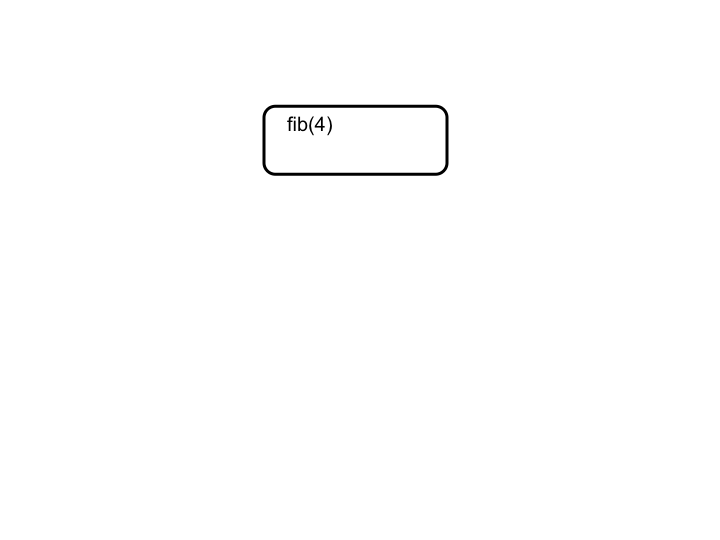
\includegraphics[width=0.7\columnwidth]{./assets/Slide039.png}
\caption{fibonacci algorithmus \cite{Herlihy1}[25]}
\label{fig:my_label}
\end{figure}

\end{frame}

\begin{frame}{Fibonacci Algorithmus}{Multithreading Analyse}

\begin{figure}
\centering
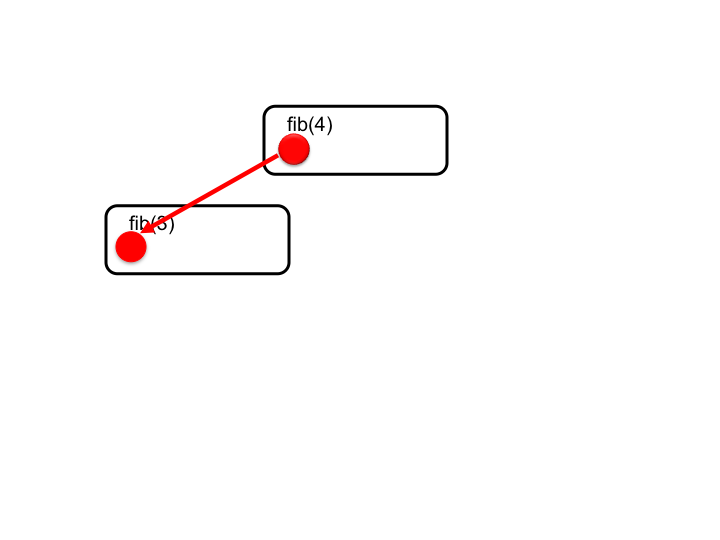
\includegraphics[width=0.7\columnwidth]{./assets/Slide040.png}
\caption{fibonacci algorithmus \cite{Herlihy1}[25]}
\label{fig:my_label}
\end{figure}

\end{frame}

\begin{frame}{Fibonacci Algorithmus}{Multithreading Analyse}

\begin{figure}
\centering
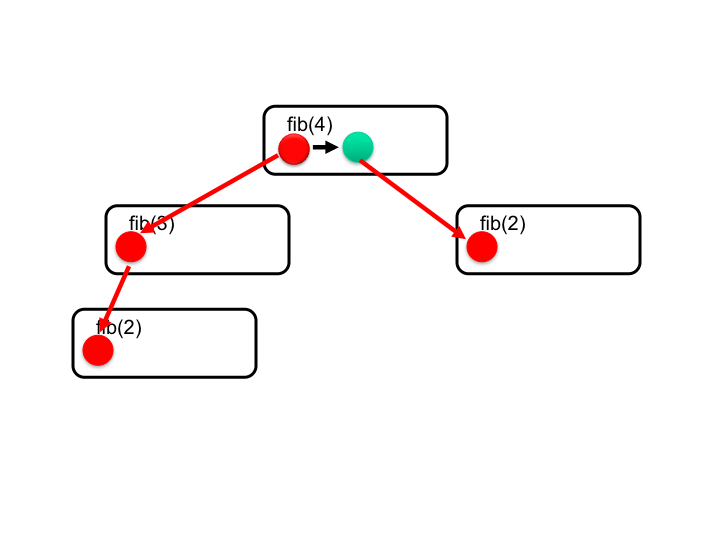
\includegraphics[width=0.7\columnwidth]{./assets/Slide041.png}
\caption{fibonacci algorithmus \cite{Herlihy1}[25]}
\label{fig:my_label}
\end{figure}

\end{frame}


\begin{frame}{Fibonacci Algorithmus}{Multithreading Analyse}

\begin{figure}
\centering
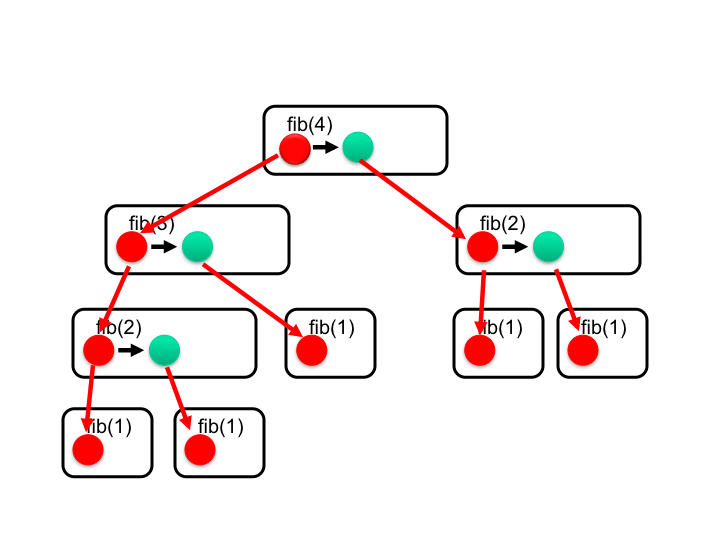
\includegraphics[width=0.7\columnwidth]{./assets/Slide042.png}
\caption{fibonacci algorithmus \cite{Herlihy1}[25]}
\label{fig:my_label}
\end{figure}

\end{frame}

\begin{frame}{Fibonacci Algorithmus}{Multithreading Analyse}

\begin{figure}
\centering
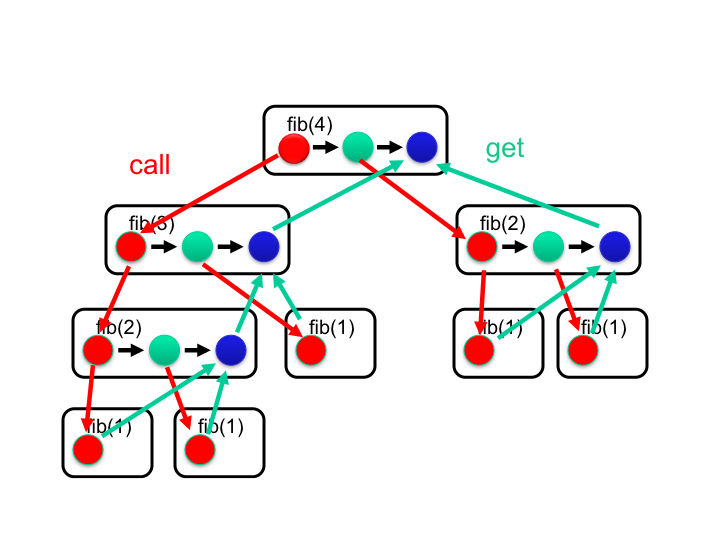
\includegraphics[width=0.7\columnwidth]{./assets/Slide043.png}
\caption{fibonacci algorithmus \cite{Herlihy1}[25]}
\label{fig:my_label}
\end{figure}

\end{frame}

\subsection{Multithreading als gerichteter azyklischer Graph}
\begin{frame}{Multithreading als gerichteter azyklischer Graph}{Multithreading Analyse}
\begin{itemize}
\item Multithreading als gerichteter azyklischer Graph
\item 1 Aufgabe = 1 Knoten
\item 1 Kante = 1 Abh\"angigkeit
\end{itemize}
\end{frame}

\begin{frame}{Aufgeklappter antizyklischer Graph}{Multithreading Analyse}
\begin{columns}
    \column{.4\textwidth}
        \begin{figure}
        \centering
        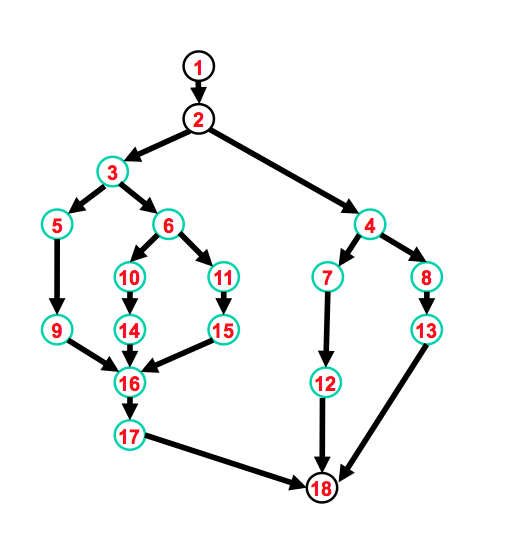
\includegraphics[width=1\columnwidth]{./assets/gag.png}
        \caption{fibonacci algorithmus \cite{Herlihy1}[25]}
        \label{fig:my_label}
        \end{figure}
    \column{.6\textwidth}
    
        \begin{itemize}
        \item Seriell: 1, 2, 18
        \item Parallel: 3, 4, ..., 17
        \end{itemize}
    
\end{columns}


\end{frame}





\subsection{Durchlaufzeit}
\begin{frame}{Durchlaufzeit}{Multithreading Analyse}
\begin{columns}
    \column{.4\textwidth}
        \begin{figure}
        \centering
        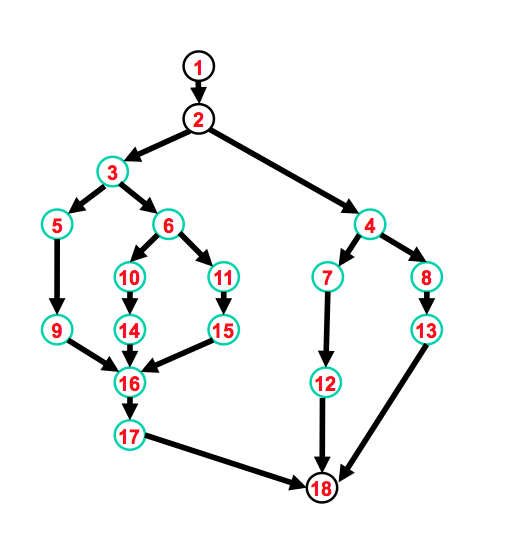
\includegraphics[width=1\columnwidth]{./assets/gag.png}
        \caption{fibonacci algorithmus \cite{Herlihy1}[25]}
        \label{fig:my_label}
        \end{figure}
    \column{.6\textwidth}
        Durchlaufzeit f\"ur n Prozessoren
        \begin{itemize}
        \item 1 Prozessor: 18
        \item 2 Prozessoren: 12
        \item unendlich viele Prozessoren / Kritischer Pfad: 9
        \end{itemize}
        
    
\end{columns}


\end{frame}

\subsection{Speedup}
\begin{frame}{Speedup}{Multithreading Analyse}
\begin{columns}
    \column{.4\textwidth}
        \begin{figure}
        \centering
        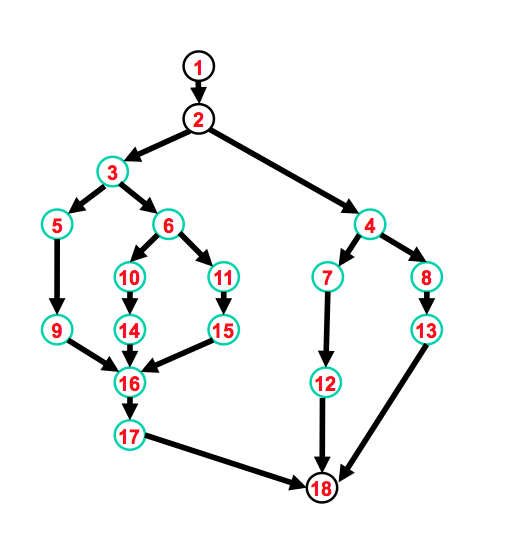
\includegraphics[width=1\columnwidth]{./assets/gag.png}
        \caption{fibonacci algorithmus \cite{Herlihy1}[25]}
        \label{fig:my_label}
        \end{figure}
    \column{.6\textwidth}
        
        
        Speedup nach Anzahl Prozessoren
        \begin{itemize}
        \item Speedup(1) = 18 / 9 = 2
        \item Speedup(2) = 12 / 9 = 1.333
        \item Speedup(max) = 9 / 9 = 1
        
        \item max = 3 Prozessoren
        \end{itemize}
    
\end{columns}
\end{frame}

\section{Realistisches Scheduling}
\subsection{Probleme durch statische Aufgabenverteilung in der Realit\"at}

\begin{frame}{Realistisches Scheduling}{Probleme durch statische Aufgabenverteilung in der Realit\"at}
\begin{columns}
    \column{.4\textwidth}
        \begin{figure}
        \centering
        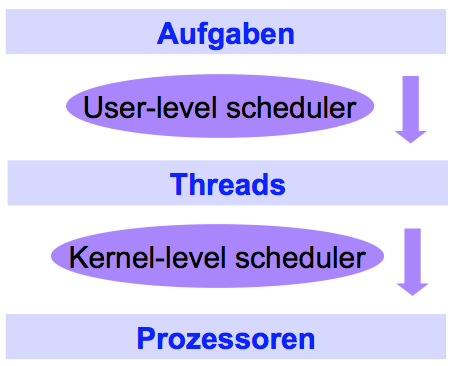
\includegraphics[width=1\columnwidth]{./assets/scheduler.png}
        \caption{Scheduling \cite{Herlihy1}[25]}
        \label{fig:my_label}
        \end{figure}
    \column{.6\textwidth}
        
        
        Realit\"at
        \begin{itemize}
        \item Kein direkter Zugriff auf Kernel-Level Scheduler
        \item Unterschiedliche Dauer der Aufgaben
        \item fluktuierende Anzahl an Prozessoren (durch andere Prozesse)
        \end{itemize}
        
        Ergebnis: Aufgaben m\"ussen w\"ahrend der Laufzeit neu verteilt werden.
    
\end{columns}
\end{frame}





\section{Arbeitsverteilung}
\subsection{Arbeitsverteilung durch besch\"aftigte Threads}

\begin{frame}{Arbeitsverteilung durch besch\"aftigte Threads}
\begin{columns}

    \column{.5\textwidth}
        Algorithmus
        \begin{enumerate}
        \item Aufgabe wird bearbeitet
        \item Andere Threads werden auf Auslastung gepr\"uft
        \item Aufgaben werden anderen Threads zugeteilt
        \end{enumerate}

    \column{.5\textwidth}
        
        
        \begin{figure}
        \centering
        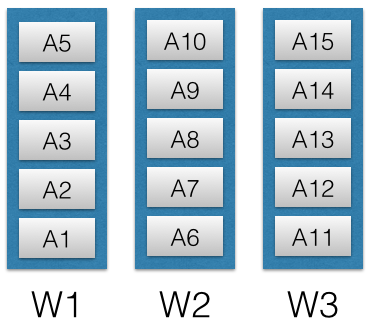
\includegraphics[width=1\columnwidth]{./assets/init.png}
        \caption{Work dealing \cite{Herlihy1}[25]}
        \label{fig:my_label}
        \end{figure}
\end{columns}
\end{frame}


\begin{frame}{Arbeitsverteilung durch besch\"aftigte Threads}
\begin{columns}

    \column{.5\textwidth}
        Algorithmus
        Algorithmus
        \begin{enumerate}
        \item Aufgabe wird bearbeitet
        \item Andere Threads werden auf Auslastung gepr\"uft
        \item Aufgaben werden anderen Threads zugeteilt
        \end{enumerate}

    \column{.5\textwidth}
        
        
        \begin{figure}
        \centering
        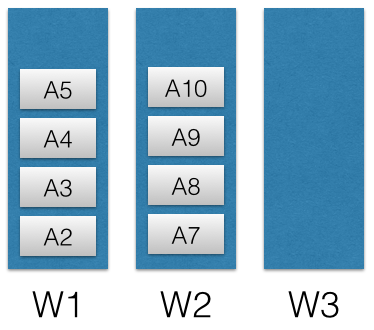
\includegraphics[width=1\columnwidth]{./assets/outOfWork.png}
        \caption{Work dealing \cite{Herlihy1}[25]}
        \label{fig:my_label}
        \end{figure}
\end{columns}
\end{frame}







\subsection{Stehlen von Aufgaben durch arbeitslose Threads}
\begin{frame}{Aufgabenneuverteilung}{Stehlen von Aufgaben durch arbeitslose Threads}
\begin{columns}

    \column{.5\textwidth}
        Algorithmus
        \begin{enumerate}
        \item Aufgabe wird bearbeitet
        \item Andere Threads werden auf Auslastung gepr\"uft
        \item Aufgaben werden anderen Threads zugeteilt
        \end{enumerate}

    \column{.5\textwidth}
        
        
        \begin{figure}
        \centering
        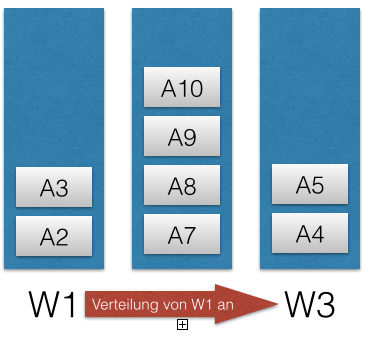
\includegraphics[width=1\columnwidth]{./assets/W1ToW3.png}
        \caption{Work dealing \cite{Herlihy1}[25]}
        \label{fig:my_label}
        \end{figure}
\end{columns}
\end{frame}


\begin{frame}{Aufgabenneuverteilung}{Neuverteilung durch arbeitenden Thread}
\begin{columns}

    \column{.6\textwidth}
        Algorithmus
        \begin{enumerate}
        \item Aufgabe wird bearbeitet
        \item Andere Threads werden auf Auslastung gepr\"uft
        \item Aufgaben werden anderen Threads zugeteilt
        \end{enumerate}

    \column{.4\textwidth}
        
        
        Probleme
        \begin{itemize}
        \item Arbeitsunterbrechung
        \item Arbeitslose Threads warten auf Zuteilung
        \end{itemize}
    
\end{columns}
\end{frame}








\begin{frame}{Aufgabenneuverteilung}{Stehlen von Aufgaben durch arbeitslose Threads}
\begin{columns}

    \column{.5\textwidth}
        Algorithmus
        \begin{enumerate}
        \item Alle Aufgaben beendet
        \item Zuf\"allige Auswahl eines anderen Threads
        \item \"Ubernahme einer Aufgabe eines anderen Threads
        \end{enumerate}

    \column{.5\textwidth}
        \begin{figure}
        \centering
        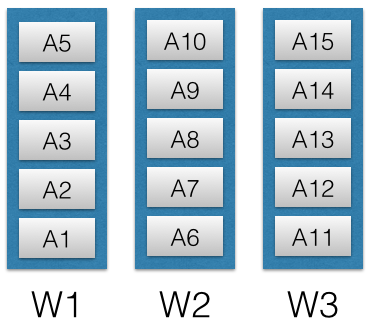
\includegraphics[width=1\columnwidth]{./assets/init.png}
        \caption{Work Stealing \cite{Herlihy1}[25]}
        \label{fig:my_label}
        \end{figure}
        
        
    
\end{columns}
\end{frame}



\begin{frame}{Aufgabenneuverteilung}{Stehlen von Aufgaben durch arbeitslose Threads}
\begin{columns}

    \column{.5\textwidth}
        Algorithmus
        \begin{enumerate}
        \item Alle Aufgaben beendet
        \item Zuf\"allige Auswahl eines anderen Threads
        \item \"Ubernahme einer Aufgabe eines anderen Threads
        \end{enumerate}

    \column{.5\textwidth}
        \begin{figure}
        \centering
        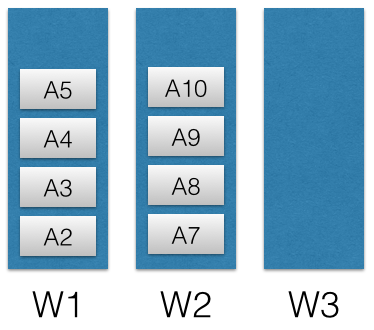
\includegraphics[width=1\columnwidth]{./assets/outOfWork.png}
        \caption{Work Stealing \cite{Herlihy1}[25]}
        \label{fig:my_label}
        \end{figure}
        
        
    
\end{columns}

\end{frame}


\begin{frame}{Aufgabenneuverteilung}{Stehlen von Aufgaben durch arbeitslose Threads}
\begin{columns}

    \column{.5\textwidth}
        Algorithmus
        \begin{enumerate}
        \item Alle Aufgaben beendet
        \item Zuf\"allige Auswahl eines anderen Threads
        \item \"Ubernahme einer Aufgabe eines anderen Threads
        \end{enumerate}

    \column{.5\textwidth}
        \begin{figure}
        \centering
        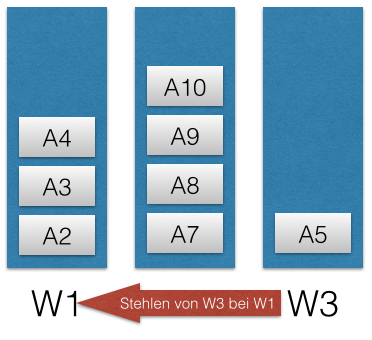
\includegraphics[width=1\columnwidth]{./assets/W3FromW1.png}
        \caption{Work Stealing \cite{Herlihy1}[25]}
        \label{fig:my_label}
        \end{figure}
        
        
    
\end{columns}
\end{frame}








\begin{frame}{Aufgabenneuverteilung}{Stehlen von Aufgaben durch arbeitslose Threads}
\begin{columns}

    \column{.5\textwidth}
        Vorteile
        \begin{itemize}
        \item keine Arbeitsunterbrechung von Arbeitenden
        \item Arbeitslose Threads weisen sich selbst Arbeit zu
        \end{itemize}

    \column{.5\textwidth}
        
        
        
        
        Probleme
        \begin{itemize}
        \item Kosten f\"ur Arbeitszuweisung
        \item \"Ubernahme von nur einer Aufgabe
        \end{itemize}
    
\end{columns}
\end{frame}


\subsection{Zentraler Aufgabenausgleich}


\begin{frame}{Aufgabenneuverteilung}{Zentraler Aufgabenausgleich}
\begin{columns}

    \column{.5\textwidth}
        Funktion
        \begin{itemize}
        \item Vergleich von Auslastung der Threads
        \item Neuverteilung bei hohen Arbeitsbelastungsdifferenzen
        \end{itemize}

    \column{.5\textwidth}
        
        
        
        
        Vorteile
        \begin{itemize}
        \item Mehere Tasks werden verschoben
        \item Ausgleich von Arbeitsbelastungsdifferenzen
        \end{itemize}
        
        Nachteil
        \begin{itemize}
        \item Threads k\"onnen arbeitslos werden
        \end{itemize}
    
\end{columns}
\end{frame}


\section{Kombination}
\subsection{Kombination von zentralem Aufgabenausgleich und Aufgaben stehlen}


\begin{frame}{Kombination}{Delegation, Zentrale Aufgabenlastverteilung, Stehlen von Arbeit}
        Vorteile
        \begin{itemize}
        \item Klare Trennung zwischen Scheduling Layern
        \item Funktionsf\"ahigkeit bei ungewisser Prozessor-Verf\"ugbarkeit
        \item OS-/ Umgebungsunabh\"angigkeit
        \end{itemize}
    
\end{frame}











%
%
%
\begin{frame}
Backup
\end{frame}



\begin{frame}{Multithreading Analyse}{Begriffe}
Begriffe:
\begin{itemize}
\item Speedup ist der erreichbare Zeit auf P Prozessoren im Vergleich zu max. vielen Prozessoren
\end{itemize}
\end{frame}














\end{document}